\documentclass[compress]{beamer}
\usepackage{ifthen,verbatim}

\newcommand{\isnote}{}
\xdefinecolor{lightyellow}{rgb}{1.,1.,0.25}
\xdefinecolor{darkblue}{rgb}{0.1,0.1,0.7}

%% Uncomment this to get annotations
%% \def\notes{\addtocounter{page}{-1}
%%            \renewcommand{\isnote}{*}
%% 	   \beamertemplateshadingbackground{lightyellow}{white}
%%            \begin{frame}
%%            \frametitle{Notes for the previous page (page \insertpagenumber)}
%%            \itemize}
%% \def\endnotes{\enditemize
%% 	      \end{frame}
%%               \beamertemplateshadingbackground{white}{white}
%%               \renewcommand{\isnote}{}}

%% Uncomment this to not get annotations
\def\notes{\comment}
\def\endnotes{\endcomment}

\setbeamertemplate{navigation symbols}{}
\setbeamertemplate{headline}{\mbox{ } \hfill
\begin{minipage}{5.5 cm}
\vspace{-0.75 cm} \small
\end{minipage} \hfill
\begin{minipage}{4.5 cm}
\vspace{-0.75 cm} \small
\begin{flushright}
\ifthenelse{\equal{\insertpagenumber}{1}}{}{Jim Pivarski \hspace{0.2 cm} \insertpagenumber\isnote/\pageref{numpages}}
\end{flushright}
\end{minipage}\mbox{\hspace{0.2 cm}}\includegraphics[height=1 cm]{../cmslogo} \hspace{0.1 cm} \includegraphics[height=1 cm]{../tamulogo} \hspace{0.01 cm} \vspace{-1.05 cm}}

\begin{document}
\begin{frame}
\vfill
\begin{center}
\textcolor{darkblue}{\Large Proposal for new MC scenario}

\vfill
\begin{columns}
\column{0.3\linewidth}
\begin{center}
\large
\textcolor{darkblue}{Jim Pivarski}
\end{center}
\end{columns}

\begin{columns}
\column{0.3\linewidth}
\begin{center}
\scriptsize
{\it Texas A\&M University}
\end{center}
\end{columns}

\vfill
29 May, 2009

\end{center}
\end{frame}

%% \begin{notes}
%% \item This is the annotated version of my talk.
%% \item If you want the version that I am presenting, download the one
%% labeled ``slides'' on Indico (or just ignore these yellow pages).
%% \item The annotated version is provided for extra detail and a written
%% record of comments that I intend to make orally.
%% \item Yellow notes refer to the content on the {\it previous} page.
%% \item All other slides are identical for the two versions.
%% \end{notes}

\small

\begin{frame}
\frametitle{First, about the data-alignment}
\scriptsize

\vspace{0.25 cm}
\mbox{\textcolor{darkblue}{Plots I showed on Monday used CRAFT\_V11 tracker geometry, rather than the new one}\hspace{-1 cm}}

\vfill
\begin{columns}
\column{0.65\linewidth}
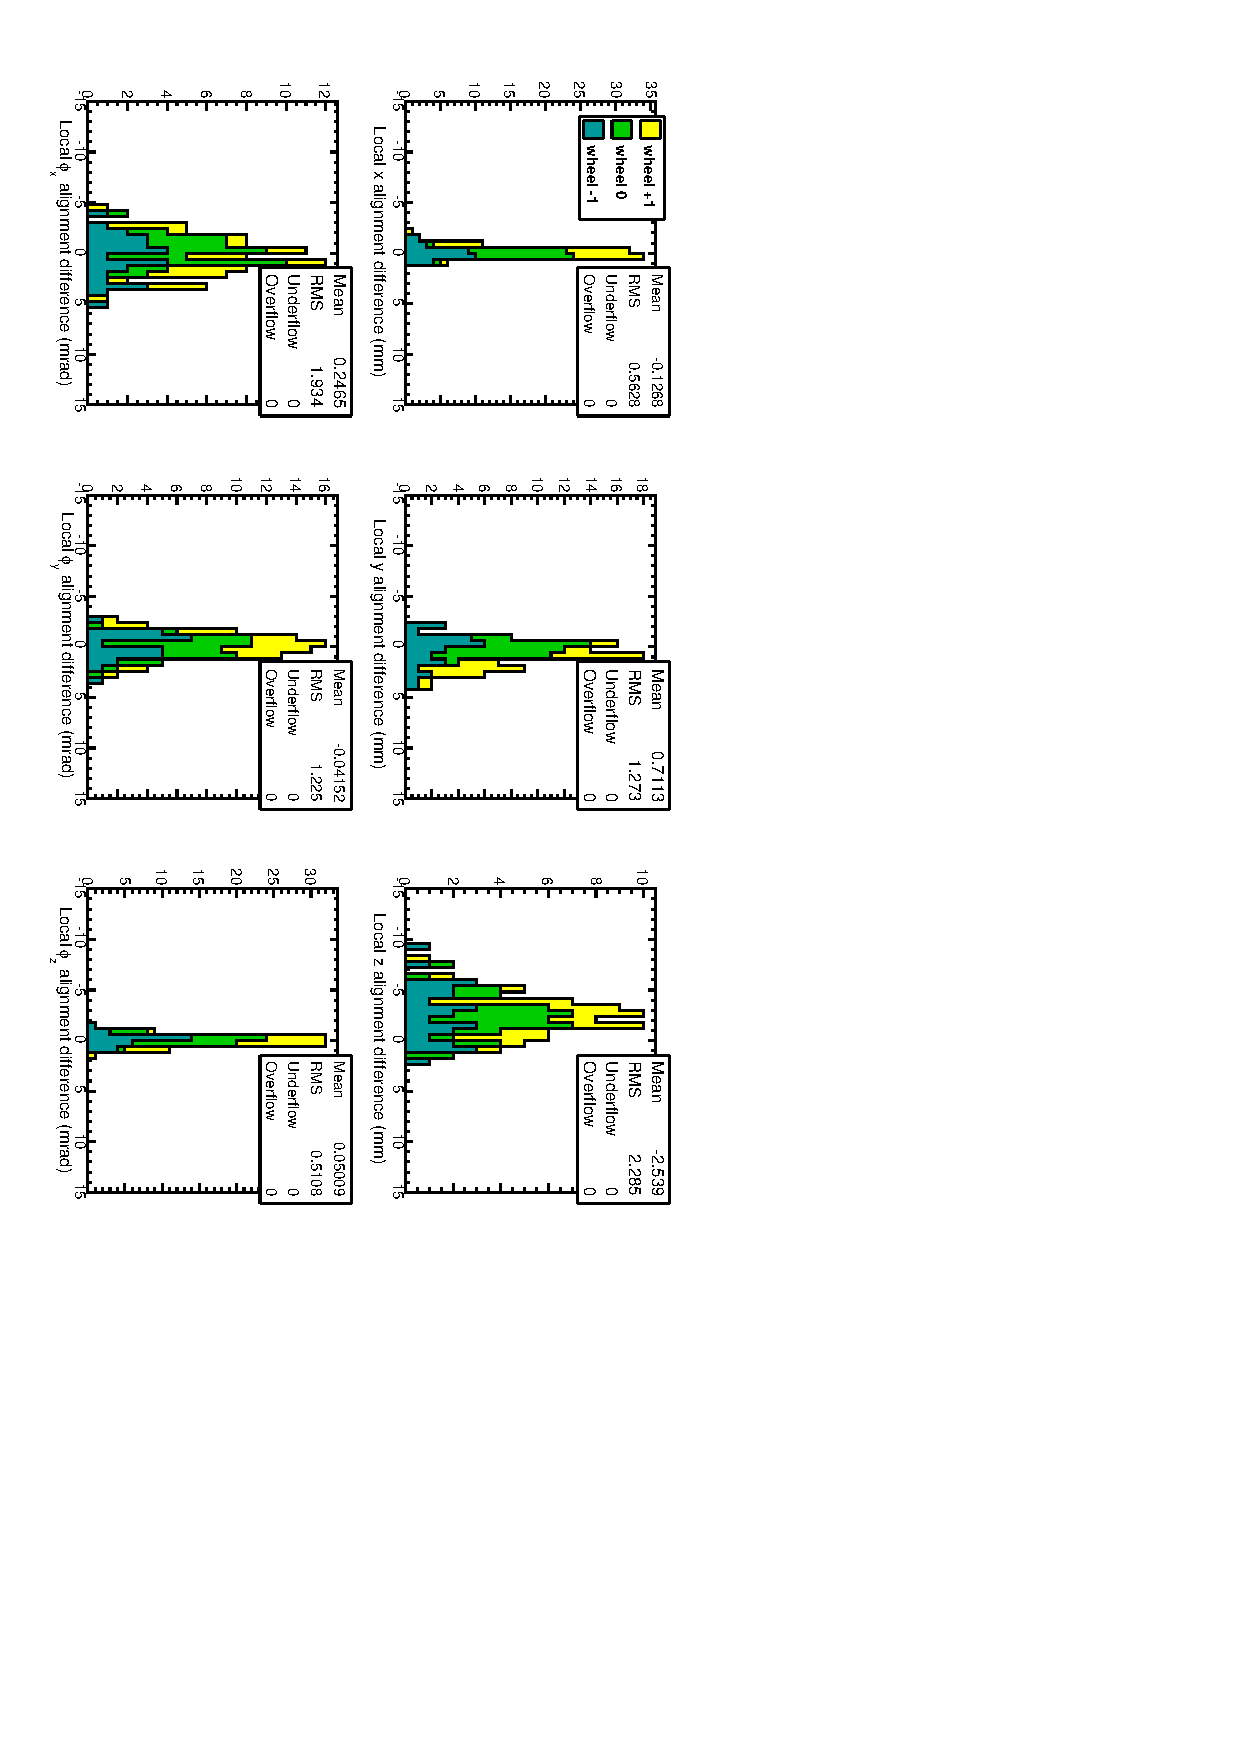
\includegraphics[height=\linewidth, angle=90]{hip_millepede_difference.pdf}
\column{0.4\linewidth}
\begin{itemize}
\item Differences between HIP and MillePede, using the same (newest) tracker geometry
\item Only 560~$\mu$m in $\delta_x$!
\item They are in \mbox{basic agreement,\hspace{-0.5 cm}} biggest differences in higher-order parameters
\end{itemize}
\vspace{0.25 cm}
\end{columns}

\vfill
\begin{columns}
\column{0.65\linewidth}
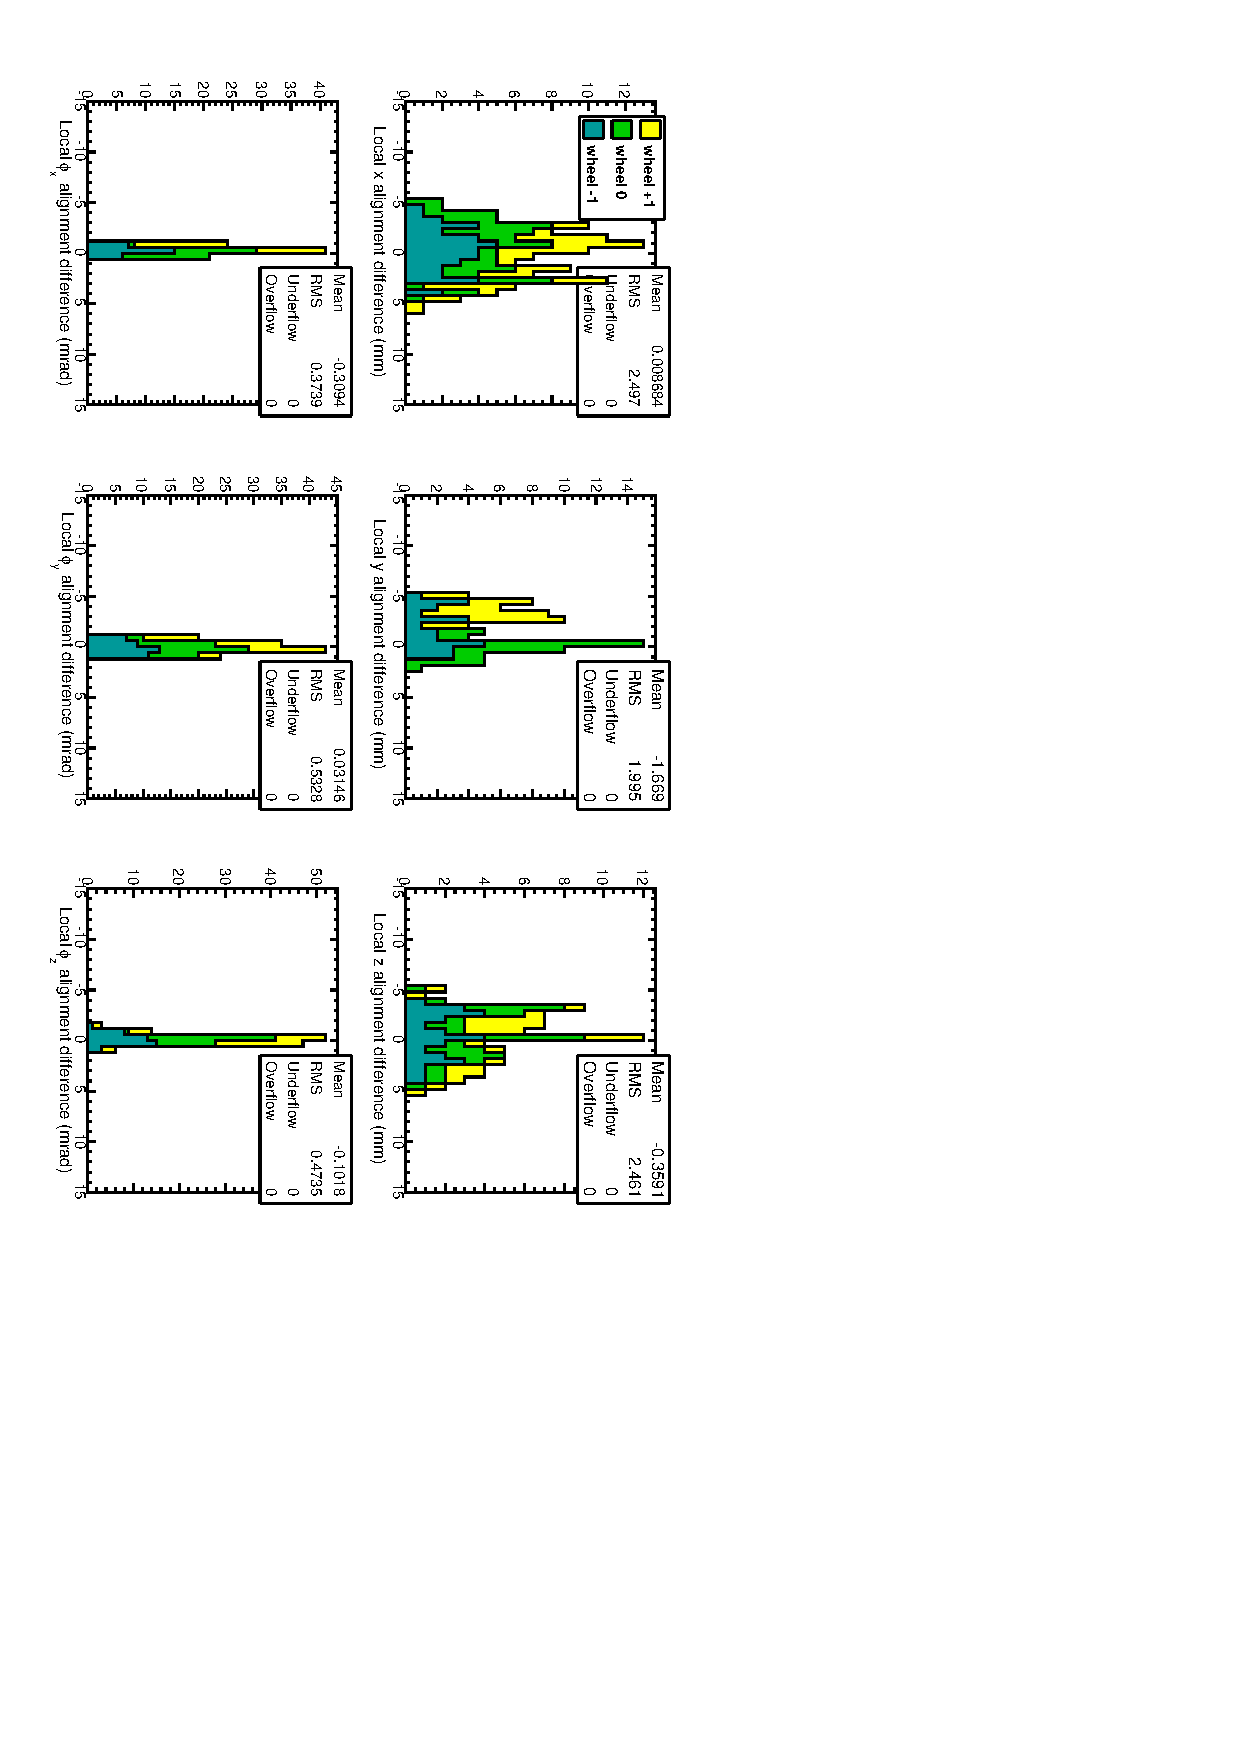
\includegraphics[height=\linewidth, angle=90]{hip_tracker_difference.pdf}
\column{0.4\linewidth}
\begin{itemize}
\item Differences between old (V11) tracker and new tracker (that which will be signed off for reprocessing)
\item 2--2.5~mm translational differences, though angular differences are small
\item Refit lost 20\% of the tracks (another indication that this tracker differs significantly)
\end{itemize}
\end{columns}
\end{frame}

\begin{frame}
\frametitle{For more information}
\begin{itemize}\setlength{\itemsep}{0.25 cm}
\item Updated slides on Monday's Indico page, can view corrections side-by-side with the original

{\tt http://indico.cern.ch/conferenceDisplay.py?confId=59610}

\item SQLite file with finalized tracker geometry {\it is} correct:

{\tt /castor/cern.ch/user/p/pivarski/

\hfill DTCRAFTiter03\_withCenteredTracker.db}

{\scriptsize (on CASTOR, use rfcp; tag name is ``DTAlignmentRcd'')}

\item I've asked for updated segment-extrapolation validation
\begin{itemize}
\item I don't expect this to change: in past experience, alignment moves
  chambers correlated along line-of-sight of tracks \\ (as would be
  expected)
\item updated plots can be sent around by HyperNews
\end{itemize}

\item I recommend the alignment above for sign-off (with APE=0)
\begin{itemize}
\item next Wednesday
\item DT alignment, CSC alignment, and MC scenario would be a combined package
\end{itemize}
\end{itemize}
\end{frame}

\begin{frame}
\frametitle{The MC scenario}
\begin{itemize}\setlength{\itemsep}{0.2 cm}
\item Two levels of hierarchy for DT chambers: independent
  misalignment within sector-groups, correlated misalignment of
  sector-groups
\item Two cases: aligned {\scriptsize (wheels $-$1, 0, $+$1, except sec.~1 and 7)} and unaligned
\item Estimated from Monte Carlo, segment-matching, and $p_T$ dependence
\item Three levels for CSC chambers: chambers within disks
  (photogrammetry), disk-bending (SLM), and disk
  positions (tracks)
\item Estimated from photogrammetry uncertainty, comparison of DCOPS
  with photogrammetry, $\phi_y$ from beam-halo measurements
\item Also, layer uncertainties from DT track-survey comparisons and
  CSC beam-halo measurements
\end{itemize}
\end{frame}

\begin{frame}
\frametitle{Aligned DT chambers}
\begin{itemize}
\item Uncertainty within sectors

\begin{tabular}{c c c c}
$x$ $\sim$ 0.8~mm & segment-matching & $\phi_x$ $\sim$ 0.7~mrad & from MC \\
$y$ $\sim$ 1~mm & from MC & $\phi_y$ $\sim$ 0.7~mrad & segment-matching \\
$z$ $\sim$ 1~mm & from MC & $\phi_z$ $\sim$ 0.3~mrad & from MC
\end{tabular}

\mbox{\hspace{-1.75 cm}
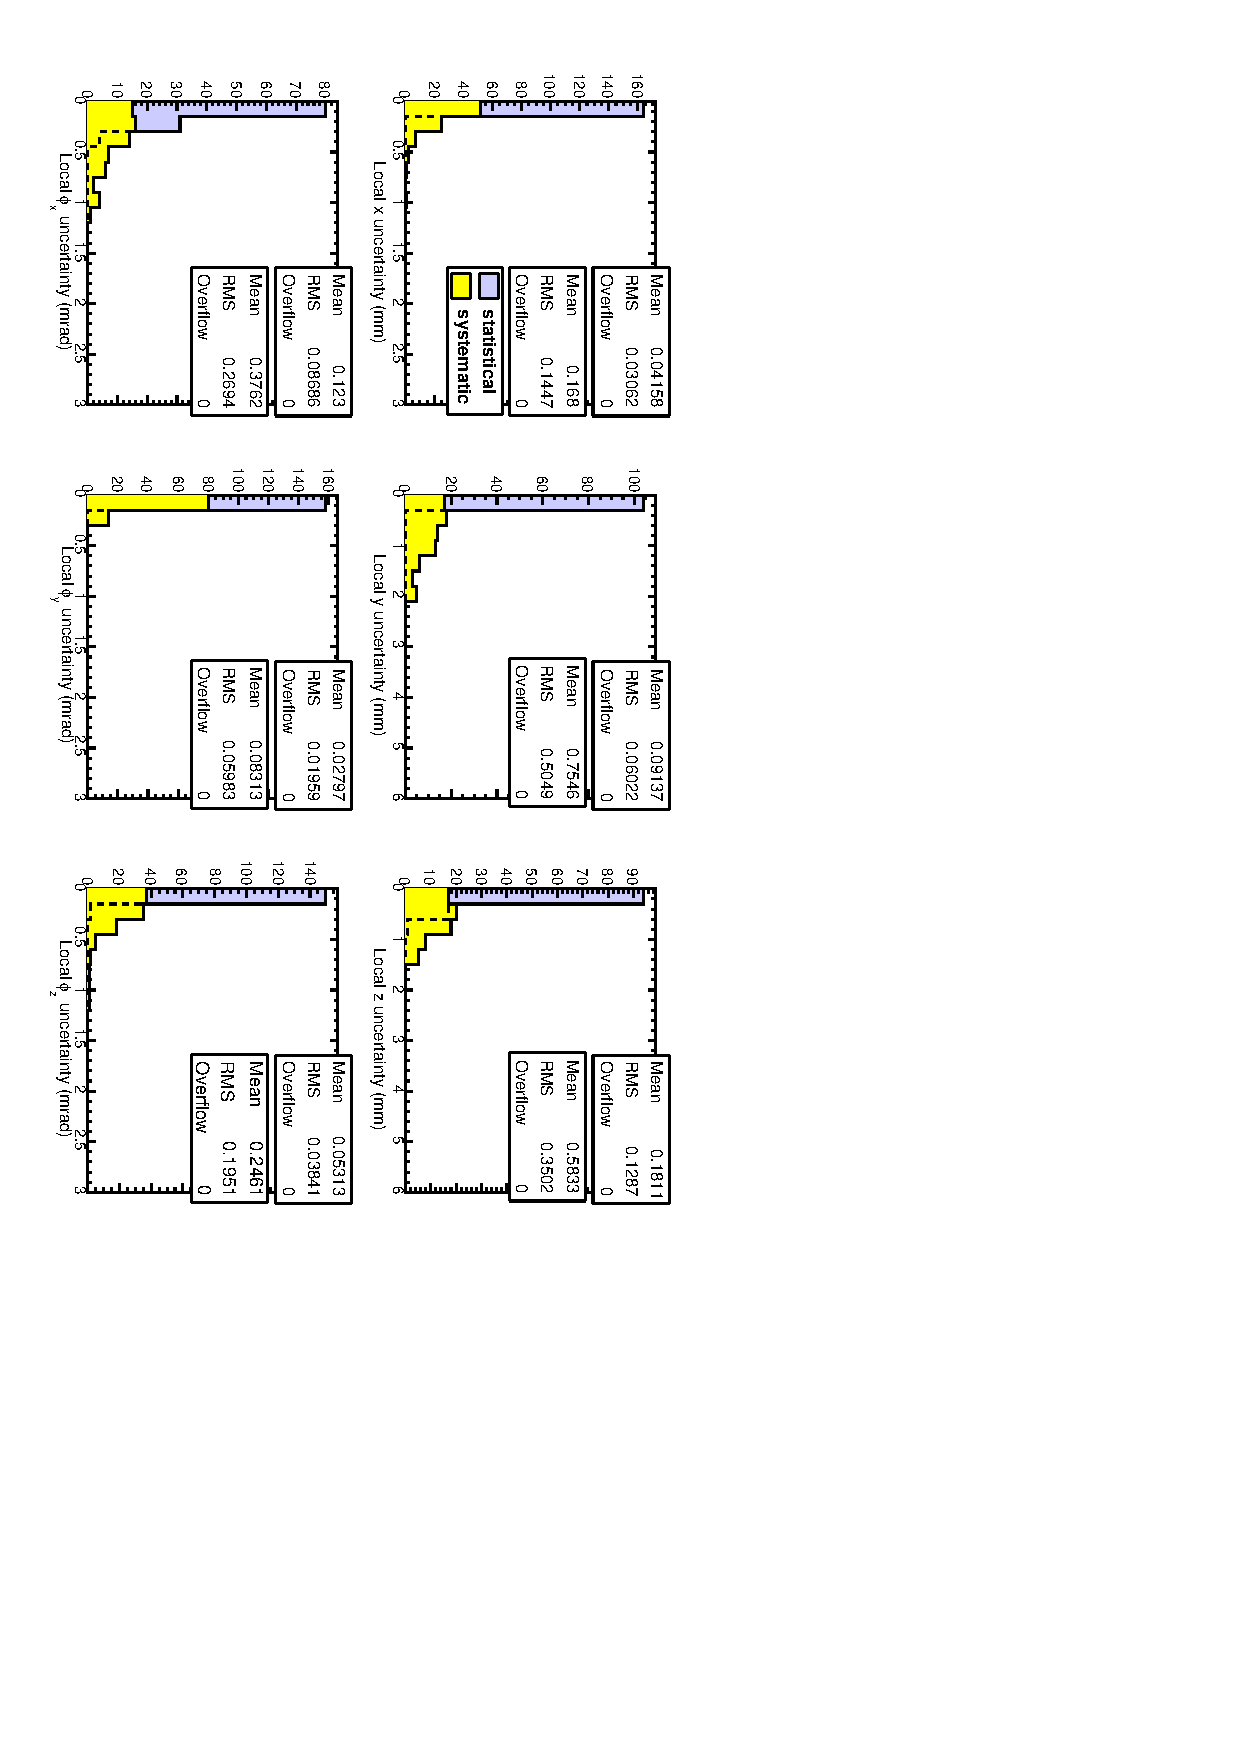
\includegraphics[height=0.8\linewidth, angle=90]{hip_MCuncertainties.pdf}
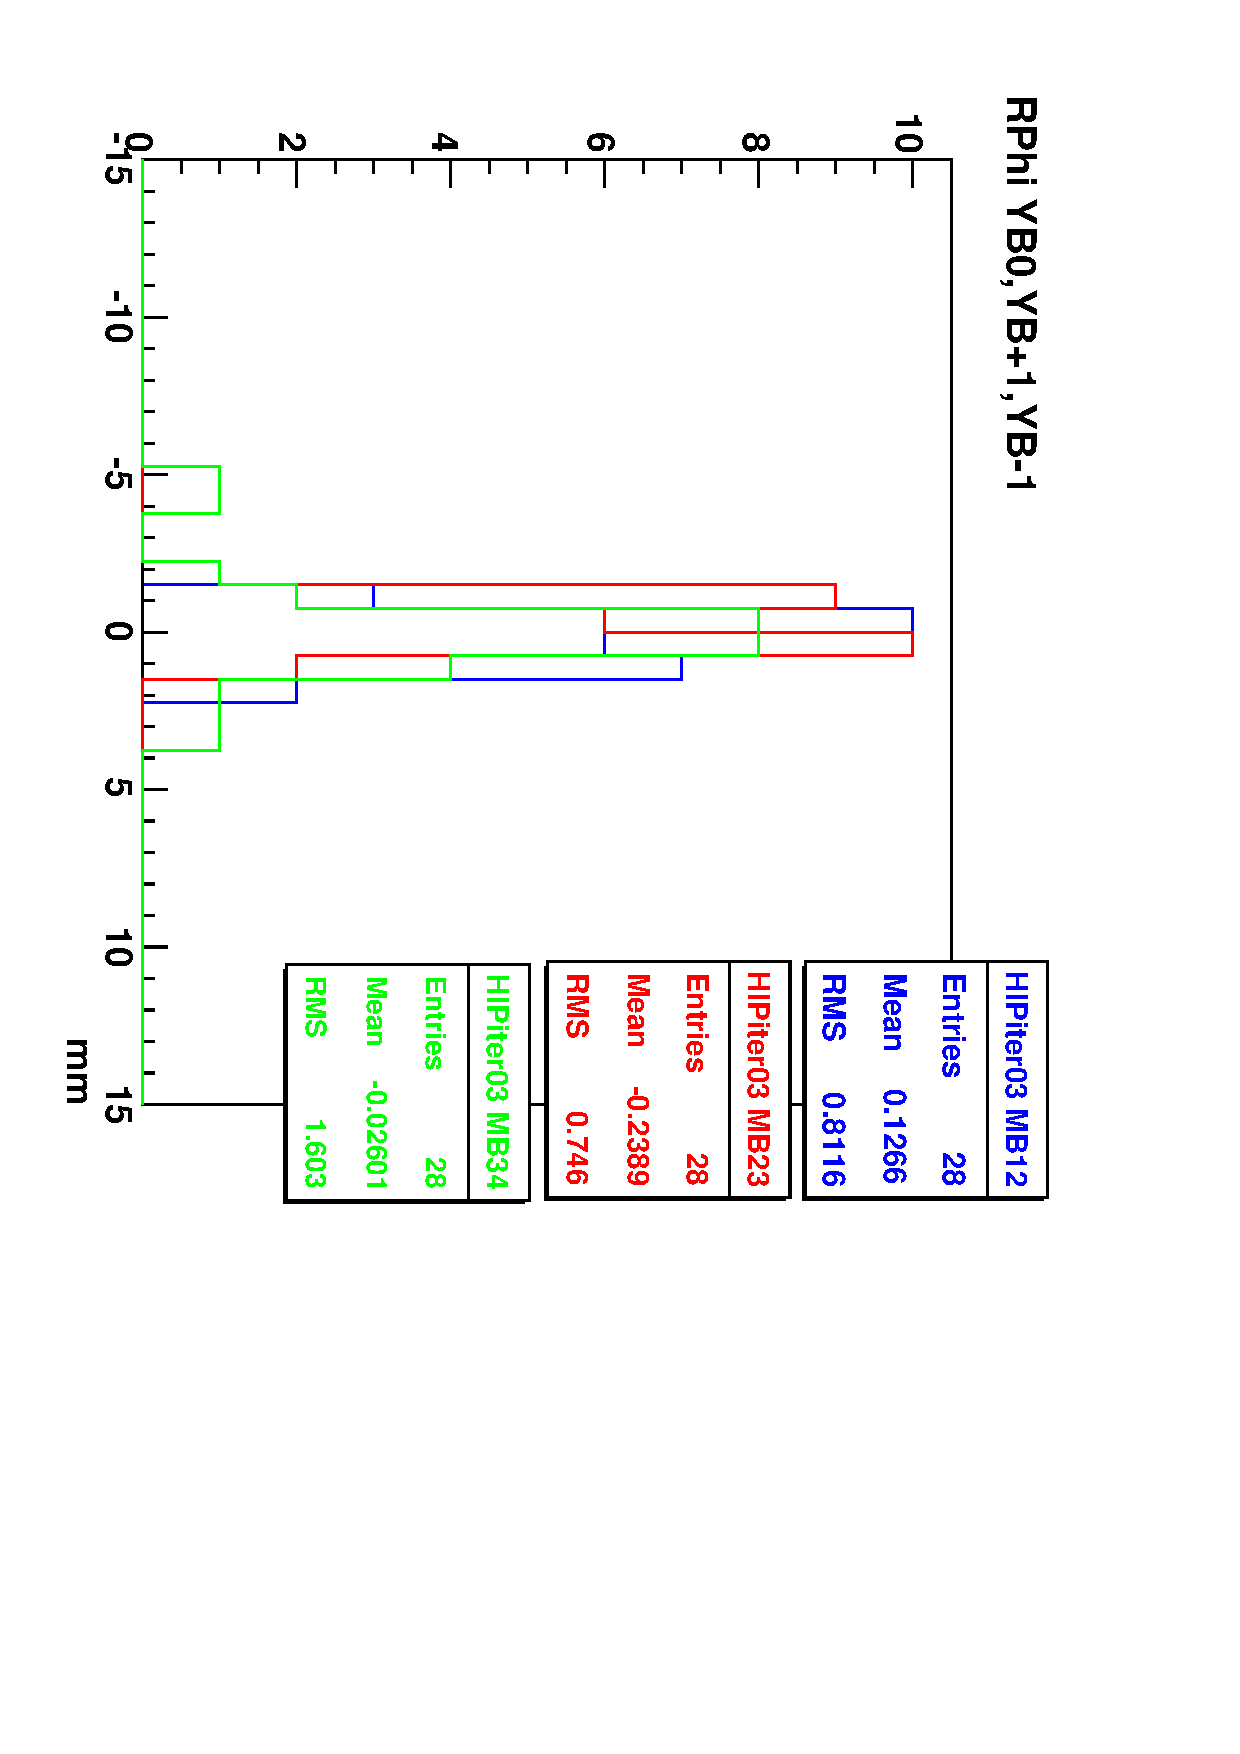
\includegraphics[height=0.4\linewidth, angle=90]{RPhires_YB0YB1YBm1_HIPiter03_InOut_38T-1.pdf}}
% 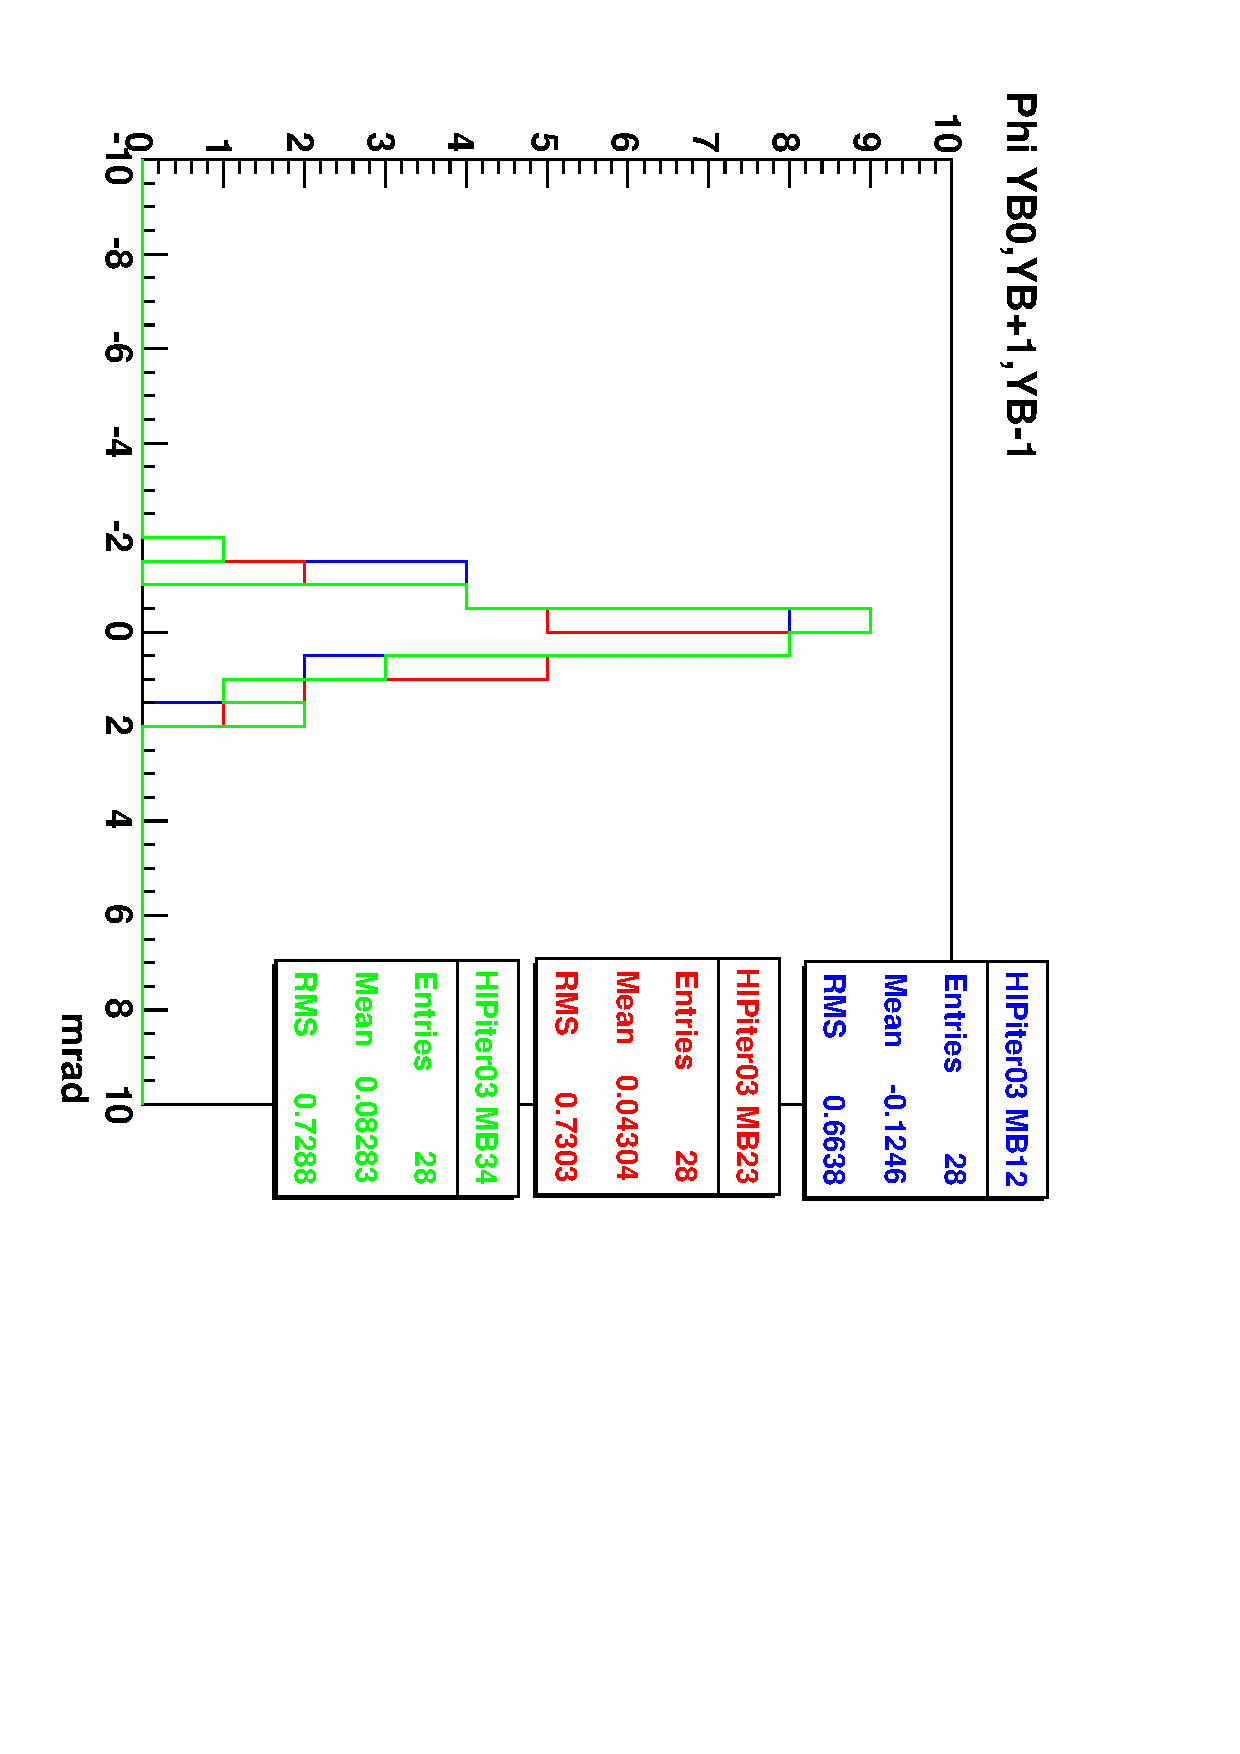
\includegraphics[height=0.35\linewidth, angle=90]{Phires_YB0YB1YBm1_HIPiter03_InOut_38T-1.pdf}}

\vspace{0.5 cm}
\item Uncertainty of sector-groups: $x$ $\sim$ 0.5~mm from track source (e.g.~$p_T$ dependence)
\end{itemize}
\end{frame}

\begin{frame}
\frametitle{Unaligned DT chambers}
\begin{itemize}
\item Uncertainty within sectors

\mbox{\hspace{-0.5 cm}\begin{tabular}{c c c c}
$x$ $\sim$ 0.8~mm & same as aligned & $\phi_x$ $\sim$ 1.6~mrad & from alignment \\
$y$ $\sim$ 2.4~mm & from alignment & $\phi_y$ $\sim$ 2.1~mrad & from alignment \\
$z$ $\sim$ 4.2~mm & from alignment & $\phi_z$ $\sim$ 1~mrad & from alignment \\
with $-$3.5~mm bias & & &
\end{tabular}}

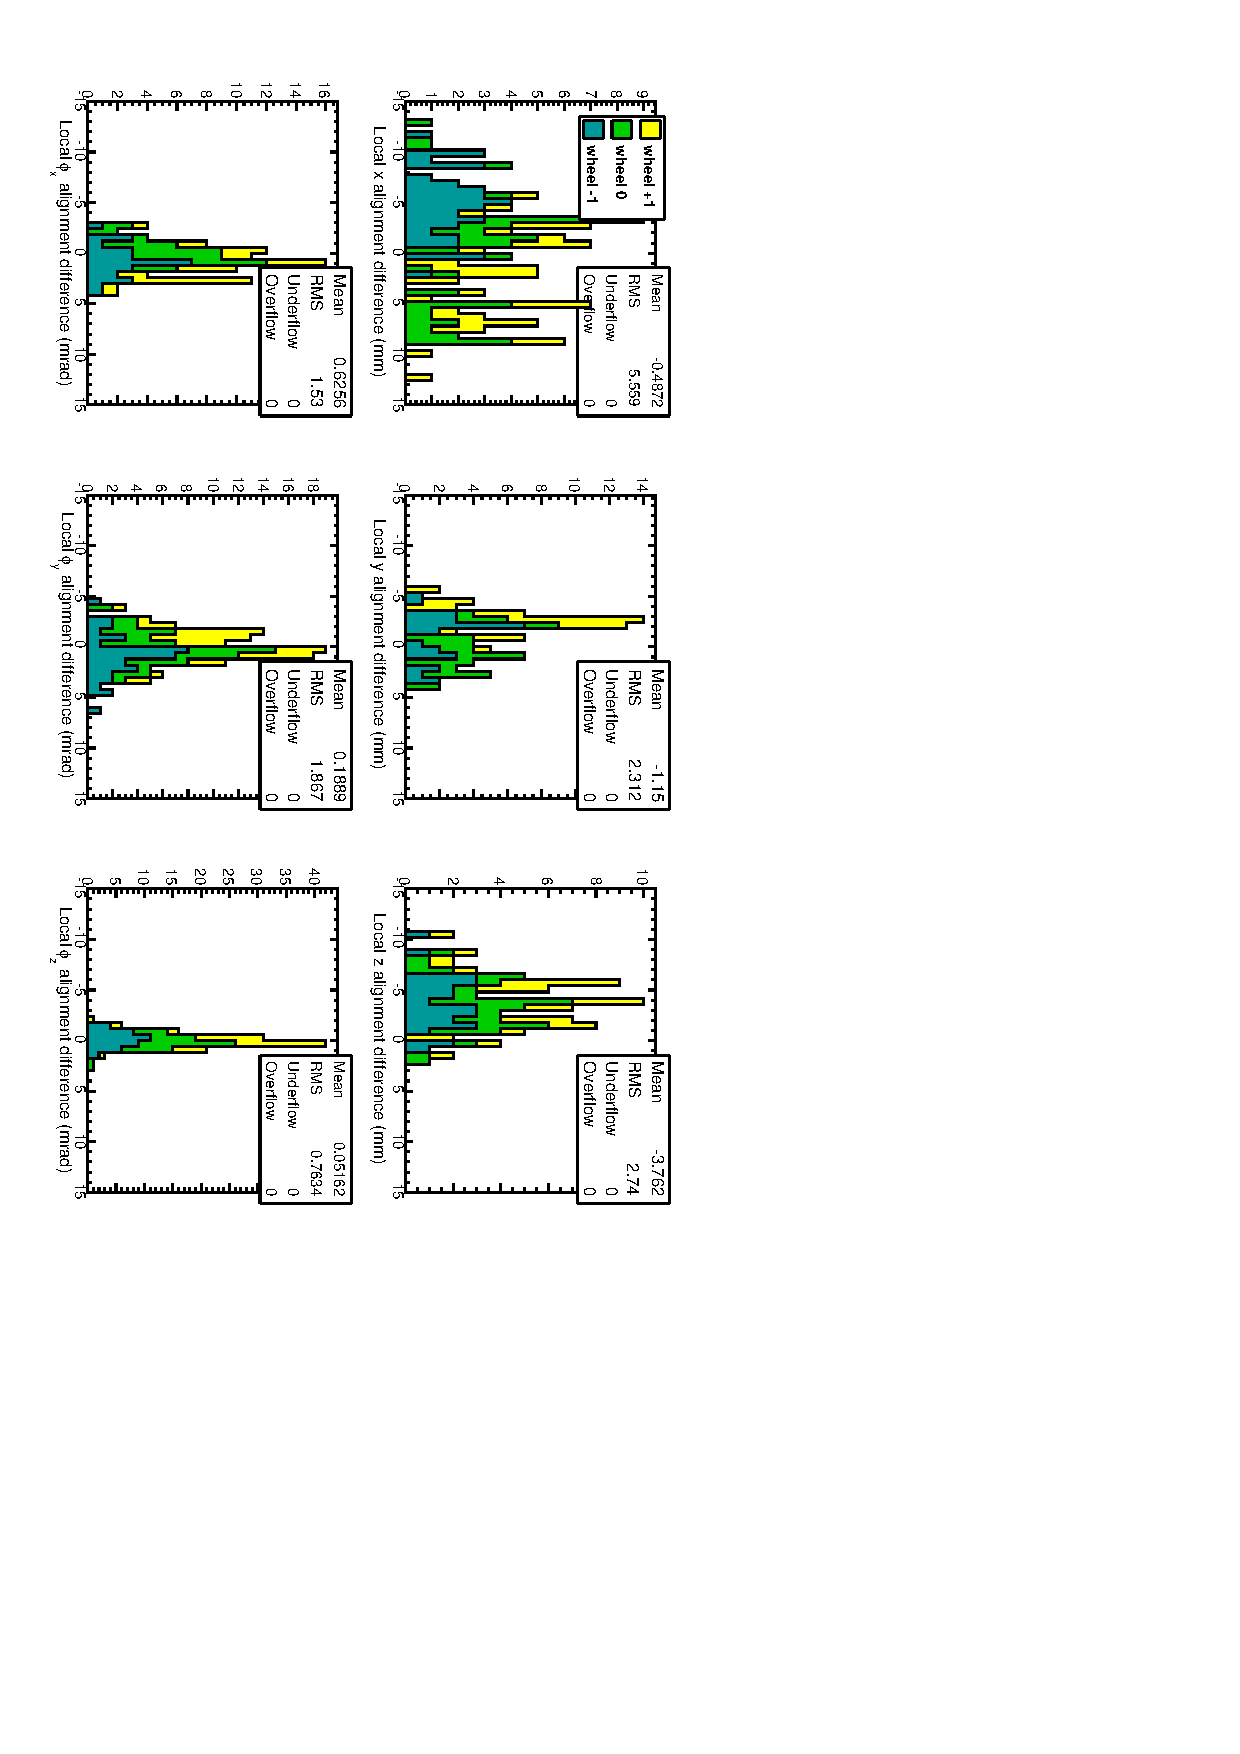
\includegraphics[height=\linewidth, angle=90]{hip_difference_v4.pdf}

\item Uncertainty of unaligned sector-groups: $x$ $\sim$ 6.5~mm
\end{itemize}
\end{frame}

\begin{frame}
\frametitle{CSC uncertainty}
\begin{itemize}\setlength{\itemsep}{0.25 cm}
\item Chambers relative to disks: photogrammetry, 0.3~mm isotropic,
  0.15~mrad $\phi_z$ rotations (from pins and length of chambers)
\item 2.3~mrad $\phi_y$ rotations observed in beam-halo tracks

\mbox{\hspace{-1 cm}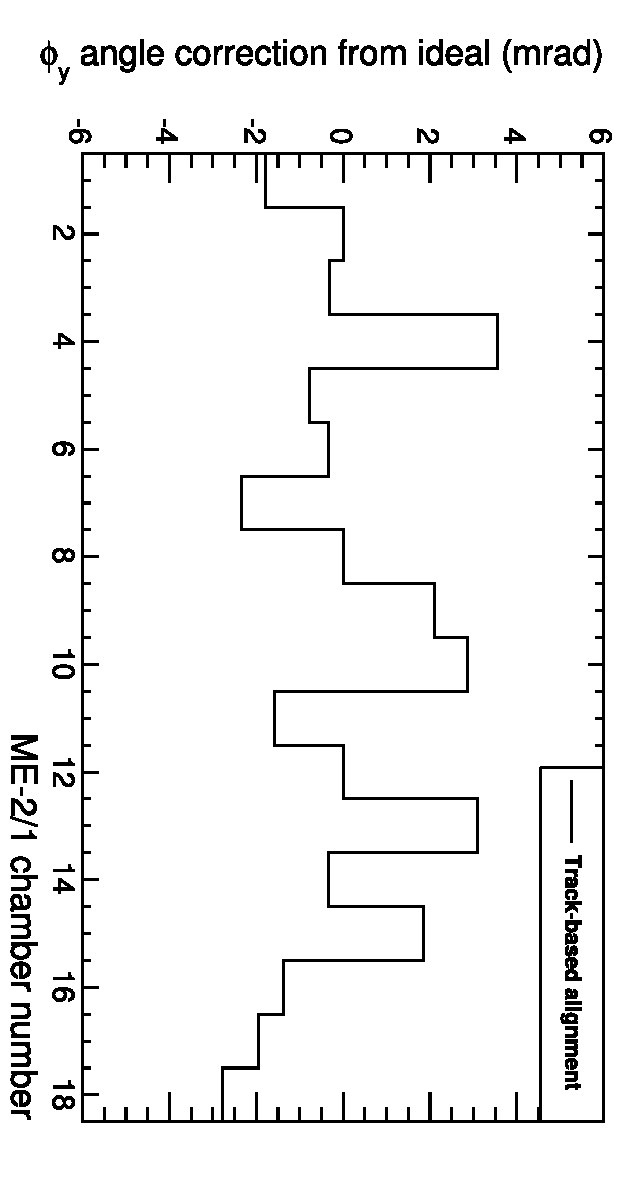
\includegraphics[height=0.6\linewidth, angle=90]{compare_m21_phiy.pdf}
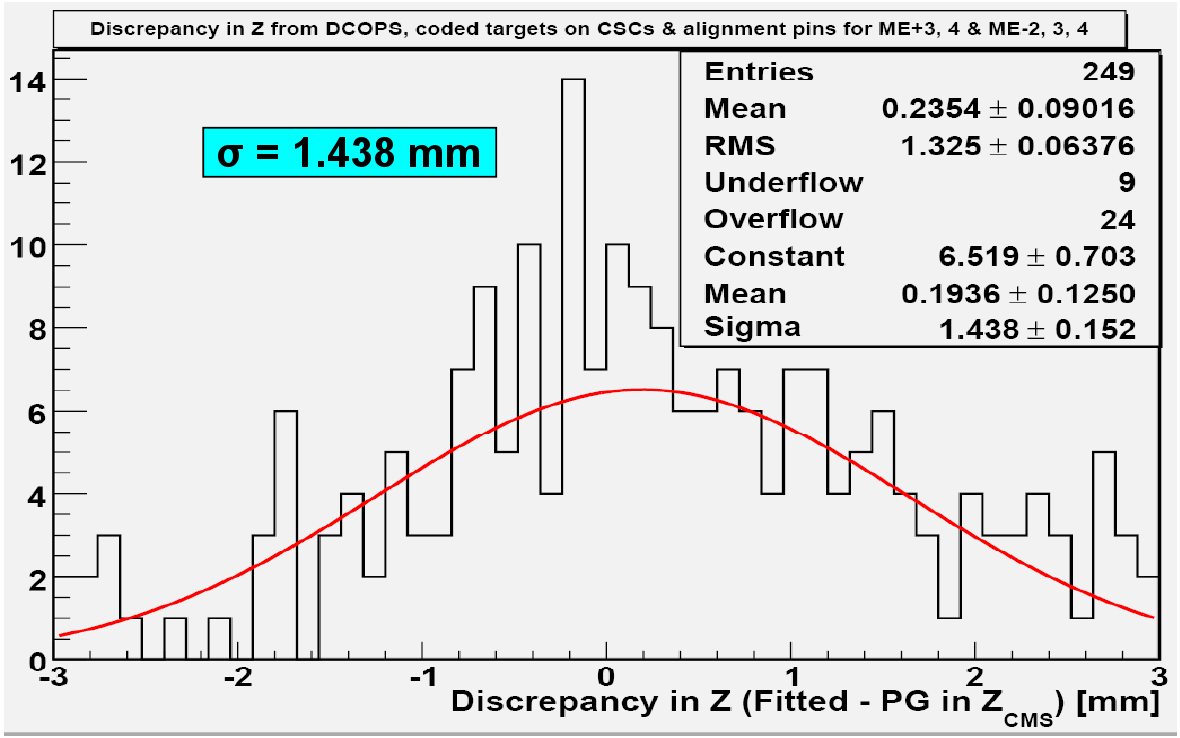
\includegraphics[width=0.5\linewidth]{dcops_in_z_replacement.png}}

\item Disk-bending ($z$ and $\phi_x$): 1.438~mm and 0.57~mrad
  uncertainty from agreement between DCOPS and photogrammetry at 0~T
\item Disk position/rotation: 0.5~mm and 0.1~mrad (after track alignment)
\end{itemize}
\end{frame}

\begin{frame}
\frametitle{Layer misalignments}

\begin{itemize}
\item DT superlayer misalignment: 0.54~mm in $z$ from track/survey comparison

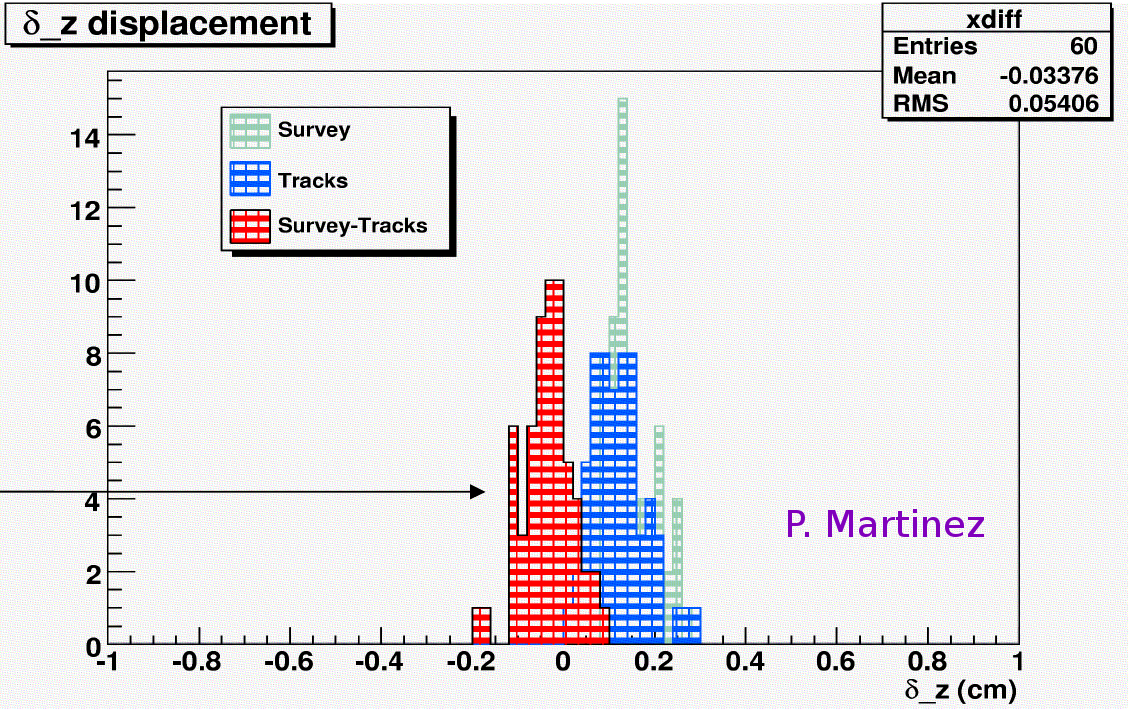
\includegraphics[width=0.6\linewidth]{internal_alignment.png}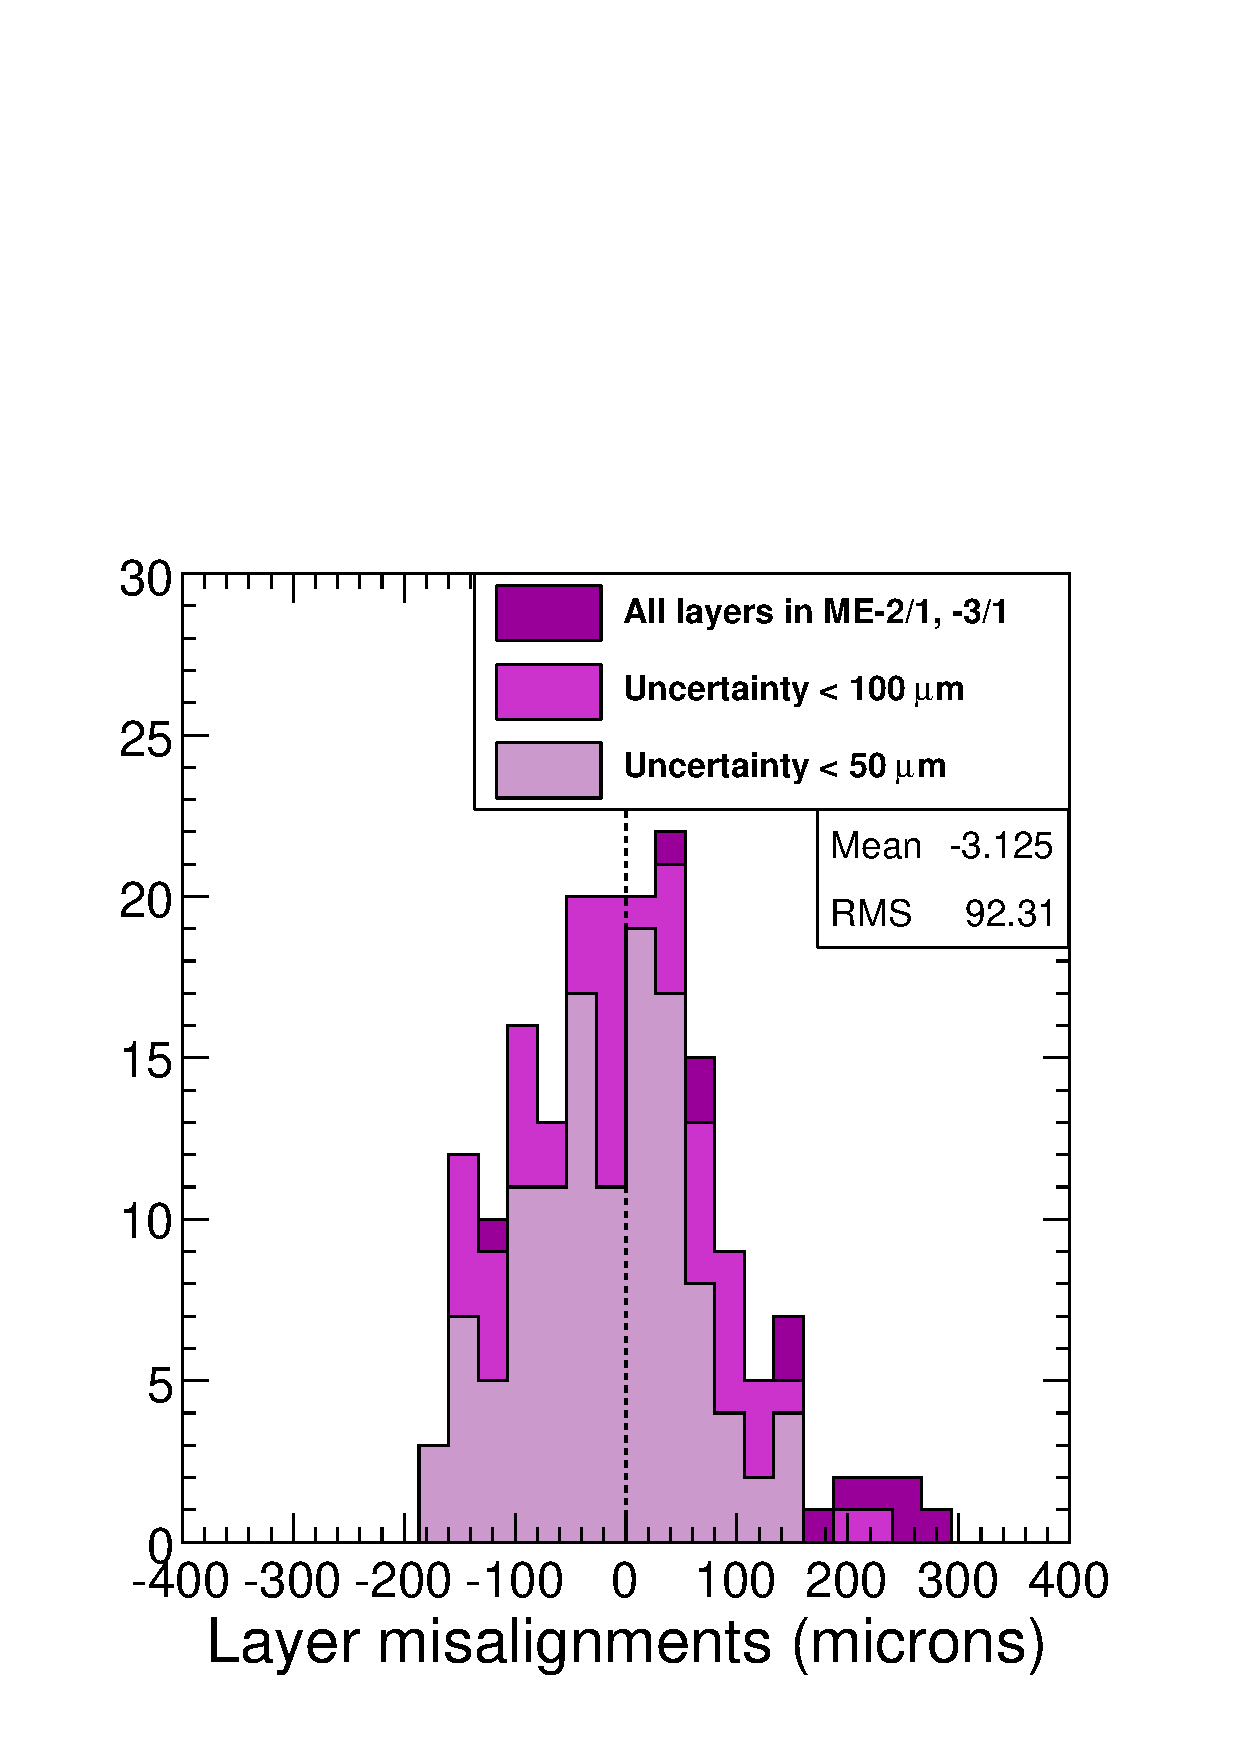
\includegraphics[width=0.4\linewidth]{layer_hist.pdf}

\item CSC layer misalignment: 0.092~mm in $x$ from beam-halo measurement
\end{itemize}
\end{frame}


%% \begin{frame}
%% \frametitle{Outline}
%% \begin{itemize}\setlength{\itemsep}{0.75 cm}
%% \item 
%% \end{itemize}
%% %% \hspace{-0.83 cm} \textcolor{darkblue}{\Large Outline2}
%% \end{frame}

%% \section*{First section}
%% \begin{frame}
%% \begin{center}
%% \Huge \textcolor{blue}{First section}
%% \end{center}
%% \end{frame}

\begin{frame}
\frametitle{Conclusions}
\begin{itemize}
\item Distribution of misalignment constants

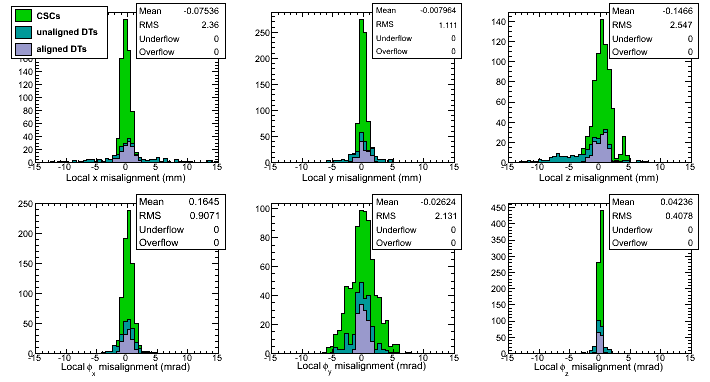
\includegraphics[width=\linewidth]{mcscenario.png}

\item Location of SQLite files on CASTOR

{\tt \scriptsize /castor/cern.ch/user/p/pivarski/MCScenario\_CRAFT1\_22X\_V02-09-04.db}

{\tt \scriptsize /castor/cern.ch/user/p/pivarski/MCScenario\_CRAFT1\_31X\_V02-09-04.db}
\end{itemize}
\label{numpages}
\end{frame}

\begin{frame}
\frametitle{Real-data disk alignments (1/2)}
\begin{itemize}
\item Optimized disk positions to reproduce plots shown by Michael Schmitt and myself
\item Michael's plots: residuals in global coordinates

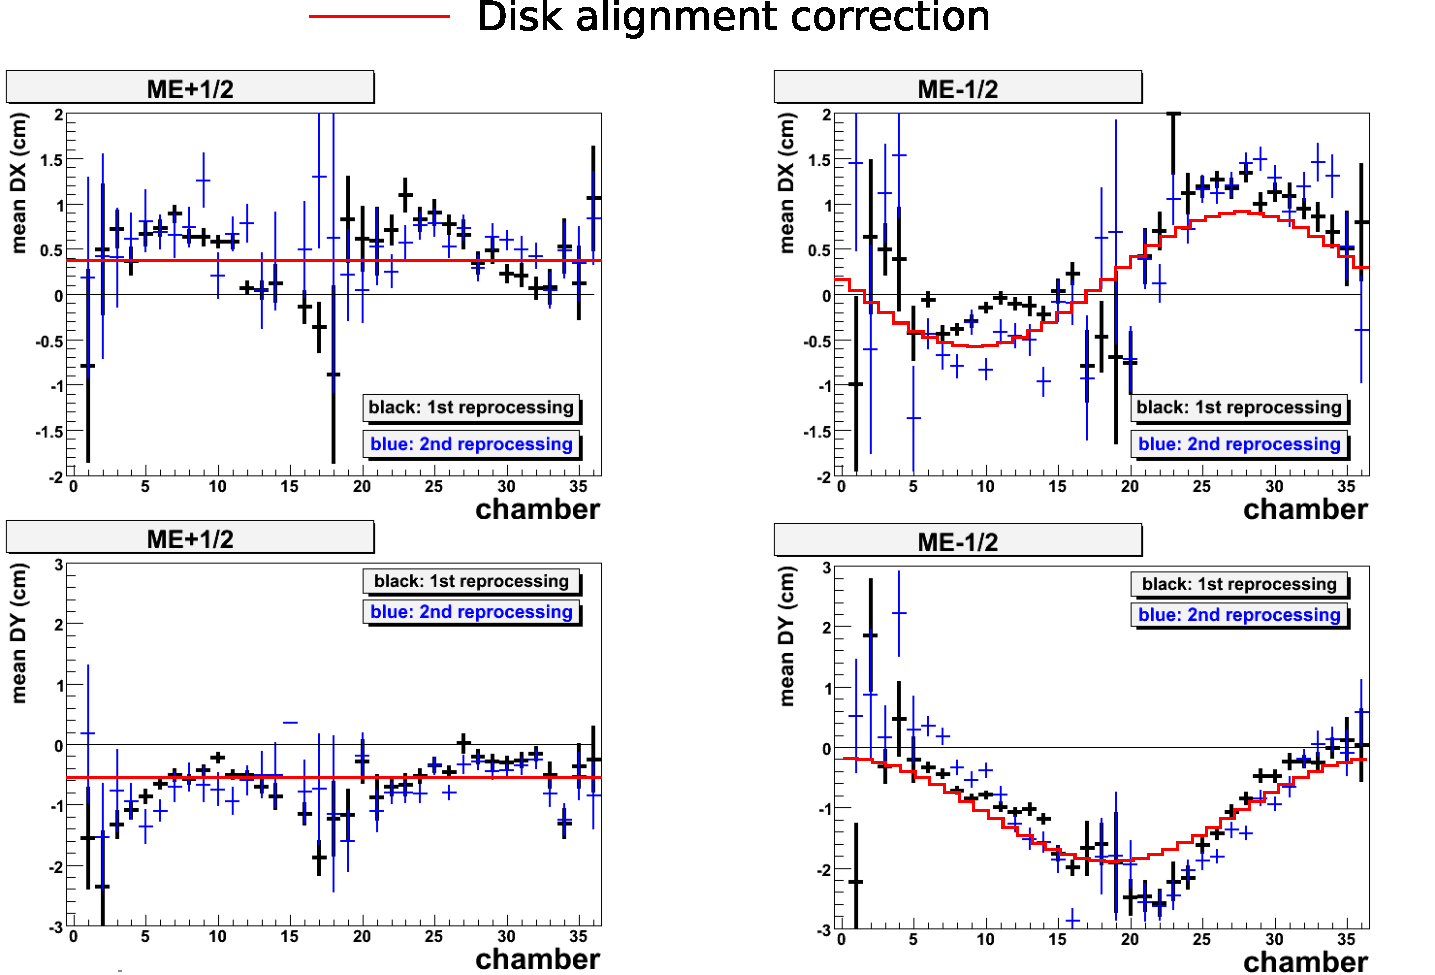
\includegraphics[width=0.85\linewidth]{Michaelsplots_globalcoords.pdf}

\item ME$-$1: 4 $x$, $-$5~mm $y$; ME$+$1: 2 $x$, $-$10~mm $y$, 2~mrad
\end{itemize}
\end{frame}

\begin{frame}
\frametitle{Real-data disk alignments (2/2)}
\begin{itemize}
\item My plots: local $x$ coordinates

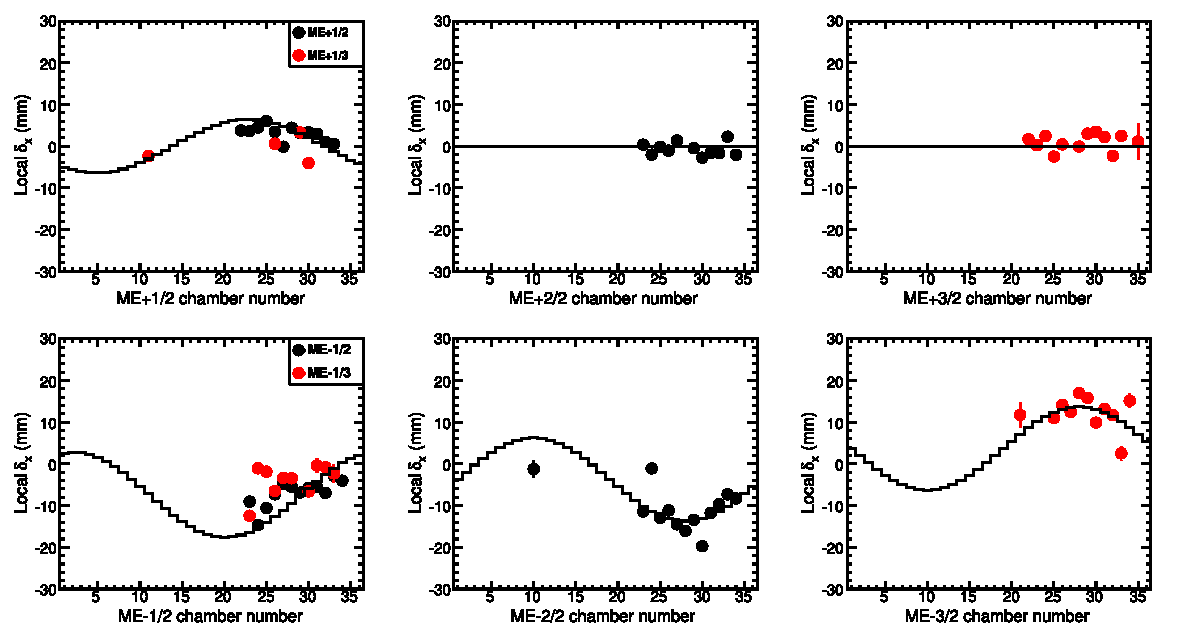
\includegraphics[width=\linewidth]{Jimsplots_localcoords.pdf}

\item Same ME$\pm$1, ME$-$2,3: 10~mm $x$, 0.7~mrad, ME$+$2,3: nothing

\item Curves produced by actual alignment scenario \mbox{implemented in CMSSW\hspace{-1 cm}}

\item Disk corrections applied on top of signed-off photogrammetry and hardware alignment
\end{itemize}
\end{frame}

\end{document}
